%============================================================
% Physics & AI (LLMs) for CFD Simulations -- compact deck
% Theme : Madrid, 16:9          Figures : ./figures/
% Build : tectonic CFD_PhysicsAI_Agentic_revised.tex
% The previous long version (50+ slides) is in git:
%   git show 72d4707:CFD_PhysicsAI_Agentic_revised.tex
%============================================================
\documentclass[aspectratio=169,10pt,t]{beamer}
\usetheme{Madrid}
\setbeamertemplate{navigation symbols}{}
\setbeamertemplate{section in toc}[sections numbered]

\usepackage[T1]{fontenc}
\usepackage{lmodern}
\usepackage{amsmath,amssymb}
\usepackage{booktabs}
\usepackage{tabularx}
\usepackage{graphicx}
\usepackage{xcolor}
\usepackage{tikz}
\usetikzlibrary{arrows.meta,positioning,calc}
\graphicspath{{figures/}}
\newcolumntype{L}{>{\raggedright\arraybackslash}X}

% ---------- colours (qblue = Madrid structure colour) ----------
\definecolor{qblue}{rgb}{0.2,0.2,0.7}
\definecolor{qorange}{RGB}{217,119,6}
\definecolor{qgreen}{RGB}{22,128,61}
\definecolor{qred}{RGB}{185,28,28}
\definecolor{qgray}{RGB}{100,110,120}
\setbeamercolor{takeaway}{fg=black,bg=qblue!10}

% ---------- helper macros ----------
\newcommand{\key}[1]{\textcolor{qblue}{\textbf{#1}}}
\newcommand{\figsrc}[1]{{\scriptsize\color{qgray}#1}}
\newcommand{\weblink}[2]{\href{#1}{\textcolor{qblue}{#2}}}
% one-line key message pinned to the bottom of a slide
\newcommand{\takeaway}[1]{%
  \par\vfill
  \begin{beamercolorbox}[wd=\linewidth,sep=5pt,rounded=true]{takeaway}
    \small\textcolor{qblue}{\textbf{Key idea:}}~#1
  \end{beamercolorbox}\vspace{1mm}}

% ---------- title ----------
\title[Physics \& AI for CFD]{Physics \& AI (LLMs) for CFD Simulations}
\subtitle{Improved PINNs for crystal growth $\cdot$ cryogenic H$_2$/N$_2$ systems $\cdot$ agentic simulation}
\author{QuaSi AI}
\date{\today}

\begin{document}

\begin{frame}[c]
\titlepage
\end{frame}

\begin{frame}{Outline}
\begin{columns}[T,onlytextwidth]
\column{0.56\textwidth}
\tableofcontents
\column{0.40\textwidth}
\begin{block}{The talk in one sentence}
\small CFD is accurate but slow and expert-heavy.
\key{Physics-informed ML} makes it fast,
\key{LLM agents} make it accessible,
and \key{validation} keeps both honest.
\end{block}
\end{columns}
\end{frame}

%============================================================
\section{Motivation}
%============================================================
\begin{frame}{Why combine physics and AI for CFD?}
\begin{columns}[T,onlytextwidth]
\column{0.48\textwidth}
\begin{block}{The bottleneck}
\begin{itemize}\small
  \item High-fidelity multi-physics CFD needs fine meshes and long runs.
  \item The real cost is the \key{sweep}: every new rotation rate, heat flux or geometry is a new simulation.
  \item Setting up a valid case needs scarce solver expertise.
\end{itemize}
\end{block}
\column{0.48\textwidth}
\begin{block}{Two complementary levers}
\begin{itemize}\small
  \item \key{Physics-informed surrogates} (PINNs, Gaussian processes): learn the solution once, then query it in milliseconds; the PDE constrains training.
  \item \key{LLM agents} (Dyad, AutoFOAM): turn a plain-language request into a runnable, checked model.
\end{itemize}
\end{block}
\end{columns}
\vspace{3mm}
\centering
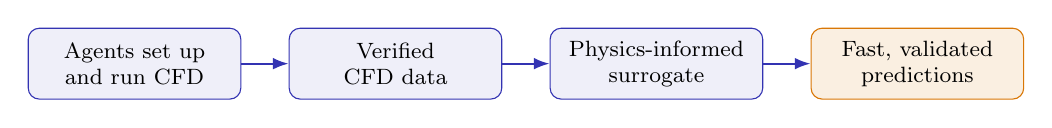
\begin{tikzpicture}[
  node distance=6mm,
  box/.style={draw=qblue,fill=qblue!8,rounded corners,minimum width=27mm,minimum height=9mm,align=center,font=\footnotesize},
  arr/.style={-{Latex[length=2mm]},thick,qblue}]
\node[box] (a) {Agents set up\\and run CFD};
\node[box,right=of a] (b) {Verified\\CFD data};
\node[box,right=of b] (c) {Physics-informed\\surrogate};
\node[box,right=of c,draw=qorange,fill=qorange!12] (d) {Fast, validated\\predictions};
\draw[arr] (a)--(b); \draw[arr] (b)--(c); \draw[arr] (c)--(d);
\end{tikzpicture}
\takeaway{Keep the governing physics, cut the cost per query, lower the set-up barrier, and always validate.}
\end{frame}

%============================================================
\section{Improved PINNs for Silicon Crystal Growth}
%============================================================
\begin{frame}{Use case: Czochralski (CZ) silicon crystal growth}
\begin{columns}[T,onlytextwidth]
\column{0.29\textwidth}
\centering
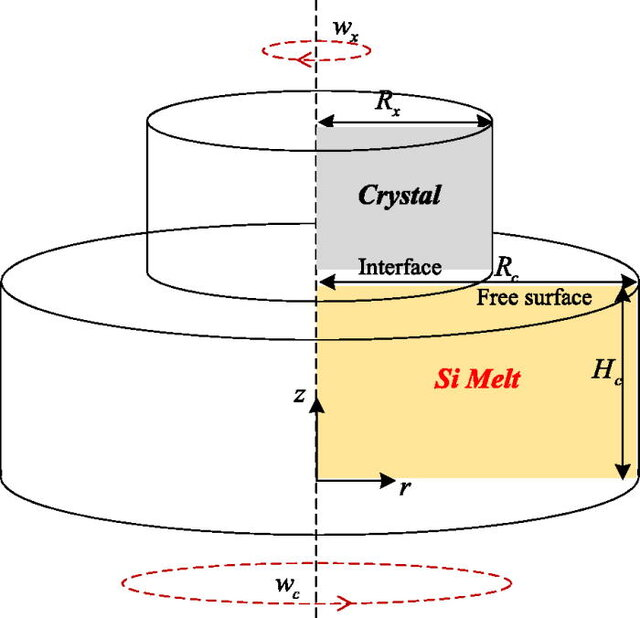
\includegraphics[width=\linewidth]{Simulation-region-of-silicon-single-crystal-growth_W640.jpg}\\[-0.5mm]
\figsrc{Axisymmetric melt domain in $(r,z)$}
\column{0.40\textwidth}
\begin{itemize}\small
  \item A seed crystal is pulled from molten silicon; crystal ($\omega_s$) and crucible ($\omega_c$) rotate.
  \item Coupled physics: Navier--Stokes + energy, Boussinesq buoyancy, rotating walls ($u_\theta=\omega r$).
  \item Five unknown fields per point: $u_r,\,u_z,\,u_\theta,\,p,\,T$.
  \item These thermal and flow fields largely determine crystal quality.
\end{itemize}
\column{0.27\textwidth}
\centering
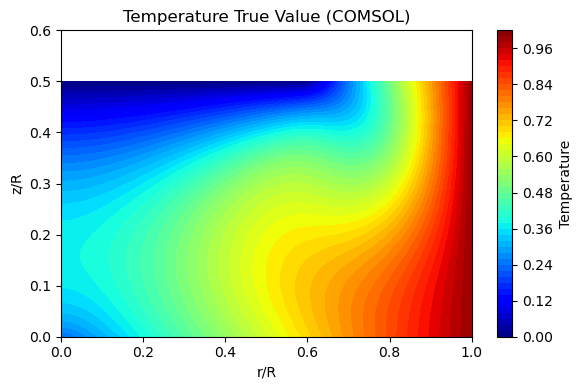
\includegraphics[height=2.35cm]{temp.png}\\
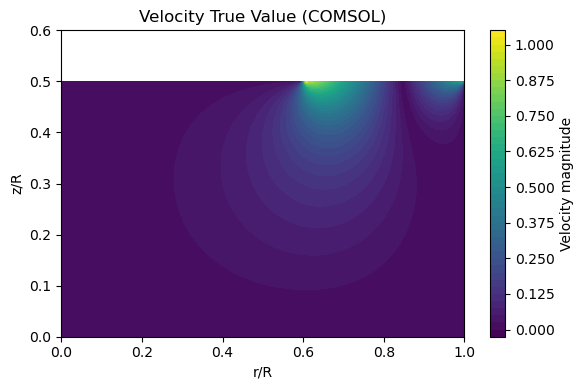
\includegraphics[height=2.35cm]{velocity.png}\\[-0.5mm]
\figsrc{Reference $T$ and $|\mathbf u|$ (normalised, COMSOL)}
\end{columns}
\takeaway{Accurate CFD exists, but sweeping process settings (rotation, heater temperature) with it is slow.}
\end{frame}

\begin{frame}{Physics-informed neural networks (PINNs) in one slide}
\begin{columns}[T,onlytextwidth]
\column{0.50\textwidth}
\centering
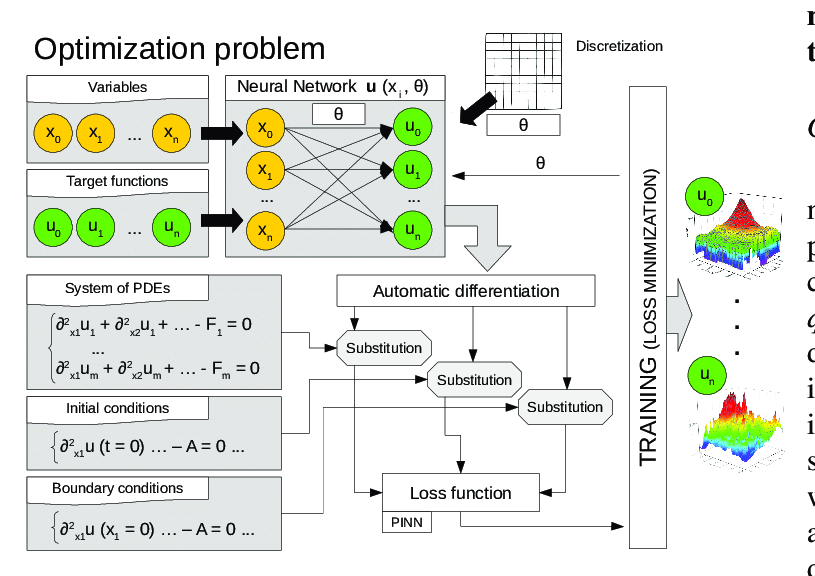
\includegraphics[width=\linewidth,height=5.0cm,keepaspectratio,trim=0 0 42 0,clip]{pinns_2.png}\\[-0.5mm]
\figsrc{Network $\rightarrow$ automatic differentiation $\rightarrow$ PDE/BC/IC residuals $\rightarrow$ loss}
\column{0.47\textwidth}
\begin{enumerate}\small
  \item A neural network $\hat u_\theta(x,t)$ represents the solution.
  \item Automatic differentiation gives exact derivatives, so the PDE residual can be evaluated at any point.
  \item One loss combines PDE, boundary (BC) and initial (IC) terms:
\end{enumerate}
\vspace{-1mm}
\[
\mathcal L=\lambda_{\mathrm{PDE}}\,\mathcal L_{\mathrm{PDE}}+\lambda_{\mathrm{BC/IC}}\,\mathcal L_{\mathrm{BC/IC}}
\]
\vspace{-3mm}
\begin{alertblock}{The catch}
\small The terms have very different gradient scales, so the weights $\lambda$ decide what the network actually learns.
\end{alertblock}
\end{columns}
\takeaway{Physics enters through the loss, so less labelled data is needed; but the loss balance must be handled with care.}
\end{frame}

\begin{frame}{Study design: two questions about trust}
\begin{columns}[T,onlytextwidth]
\column{0.48\textwidth}
\begin{block}{A.\ Adaptive PINN training}
\small \textbf{Question:} if the loss weights adapt during training, is a lower PDE loss a better solution?
\begin{itemize}\small
  \item \key{Baseline PINN}: fixed unit weights.
  \item \key{GNPINN}: normalises the PDE and BC/IC gradients.
  \item \key{AgenticPINN}: a rule-based controller re-weights the loss terms.
\end{itemize}
\small Tested on the 1D heat equation (exact solution known) and a simplified CZ thermal-fluid PINN.
\end{block}
\column{0.48\textwidth}
\begin{block}{B.\ CFD surrogate (Gaussian process)}
\small \textbf{Question:} how well does a surrogate predict a \emph{whole unseen} operating condition, field by field?
\begin{itemize}\small
  \item 33 ANSYS Fluent reference cases: steady, laminar, 2D axisymmetric, 8181 nodes.
  \item Three one-parameter sweeps: heater-wall temperature $T_{\mathrm{hot}}$, crucible rotation $\omega_c$, crystal rotation $\omega_s$.
  \item One complete case per sweep is held out for testing.
\end{itemize}
\end{block}
\end{columns}
\takeaway{Fair tests: in A only the training strategy changes; in B the test is a new process setting, not random points of known cases.}
\end{frame}

\begin{frame}{Result 1: lowest PDE residual $\neq$ best solution}
\begin{columns}[T,onlytextwidth]
\column{0.56\textwidth}
\small Heat equation $\partial_t T=\partial_{xx}T$, exact solution $T=\sin(\pi x)\,e^{-\pi^2 t}$:\\[1.5mm]
\footnotesize
\begin{tabular}{@{}lccc@{}}
\toprule
Trainer & PDE loss & BC/IC loss & Rel.\ $L_2$ error\\
\midrule
Baseline    & $3.96\times10^{-3}$ & $1.15\times10^{-3}$ & $8.43\times10^{-2}$\\
GNPINN      & $9.74\times10^{-3}$ & $\mathbf{9.05\times10^{-4}}$ & $\mathbf{5.41\times10^{-2}}$\\
AgenticPINN & $\mathbf{8.22\times10^{-7}}$ & $2.00\times10^{-1}$ & \textcolor{qred}{$\mathbf{1.368}$}\\
\bottomrule
\end{tabular}
\vspace{2mm}
\begin{itemize}\small
  \item AgenticPINN: PDE residual $\approx4800\times$ smaller, BC/IC loss $\approx173\times$ larger, and the field is wrong.
  \item Same pattern in the simplified CZ PINN: PDE residual $\approx8\times$ smaller, BC/IC loss $\approx790\times$ larger.
\end{itemize}
\column{0.41\textwidth}
\centering
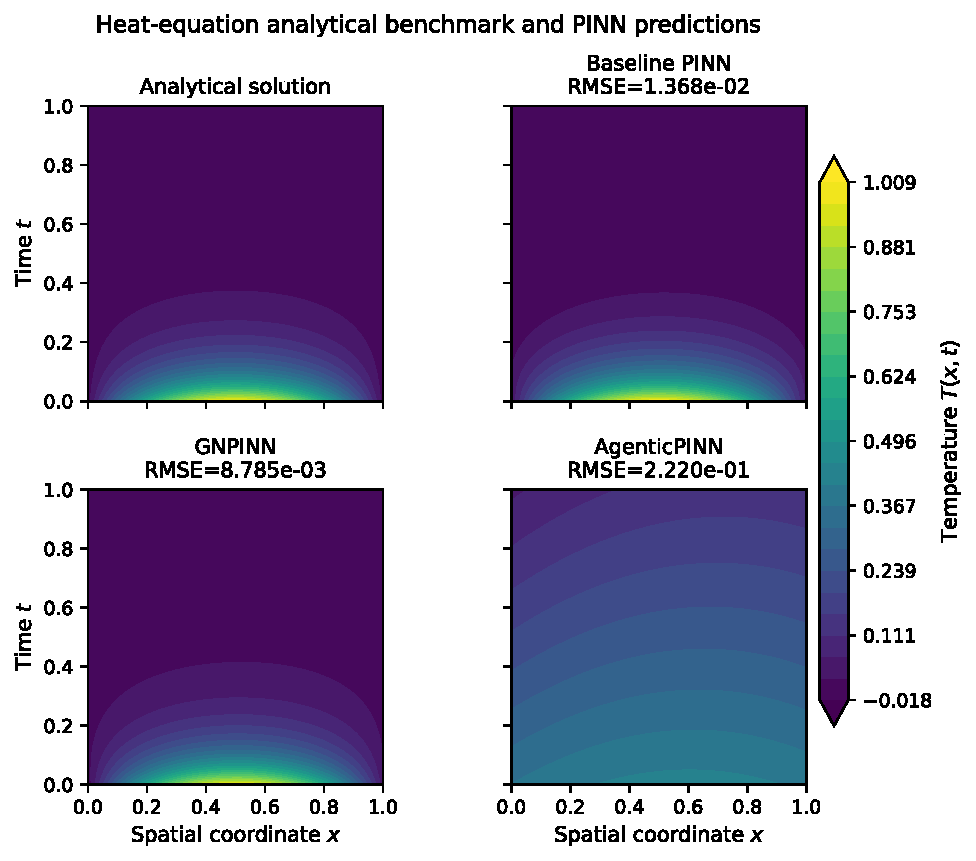
\includegraphics[width=\linewidth,height=5.0cm,keepaspectratio]{heat_mlp_method_comparison.pdf}
\end{columns}
\takeaway{Report PDE, BC and IC losses separately plus an external error; one aggregate loss can hide a failure.}
\end{frame}

\begin{frame}{Why? The controller silences the boundary conditions}
\begin{columns}[T,onlytextwidth]
\column{0.58\textwidth}
\centering
\vspace{2mm}
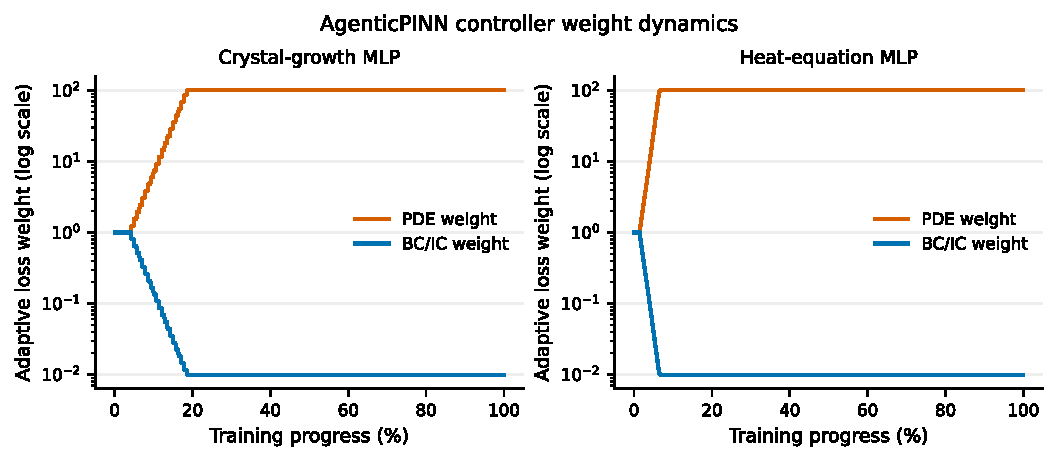
\includegraphics[width=\linewidth]{agentic_controller_dynamics_1.pdf}\\
\figsrc{AgenticPINN loss weights during training (log scale)}
\column{0.39\textwidth}
\begin{block}{Mechanism}
\small The controller balances gradient magnitudes and pushes $\lambda_{\mathrm{PDE}}\!\to\!10^{2}$ and $\lambda_{\mathrm{BC/IC}}\!\to\!10^{-2}$: a $10^4$ ratio within the first 20\% of training.
\end{block}
\begin{alertblock}{Consequence}
\small The network satisfies the PDE but no longer respects its boundary and initial conditions. Weighted total $2\times10^{-3}$ looks excellent; the relative $L_2$ error is 1.37.
\end{alertblock}
\end{columns}
\takeaway{Adaptive weighting is an optimisation tool, not an accuracy metric: always pair it with external validation.}
\end{frame}

\begin{frame}{Result 2: the surrogate's error depends on the field}
\begin{columns}[T,onlytextwidth]
\column{0.42\textwidth}
\begin{block}{Gaussian-process surrogate}
\begin{itemize}\small
  \item Learns $(r,z,s)\mapsto(u_r,u_z,u_\theta,p,T)$, where $s$ is the swept parameter.
  \item Held out: $T_{\mathrm{hot}}=1780$\,K, $\omega_c=-4$\,rpm, $\omega_s=7$\,rpm.
  \item NRMSE = RMSE / standard deviation of the field in the held-out case.
  \item Also gives a predictive uncertainty at every point.
\end{itemize}
\end{block}
\column{0.55\textwidth}
\centering
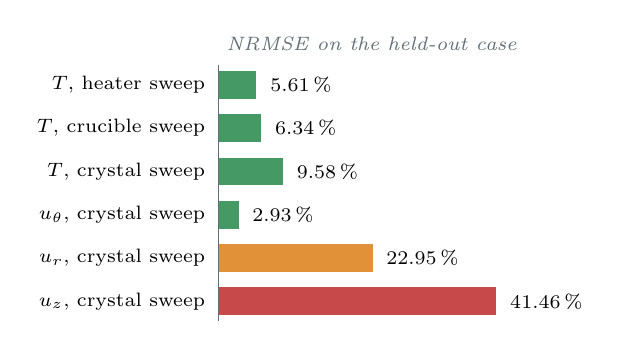
\begin{tikzpicture}[x=0.085cm,y=0.55cm,font=\scriptsize]
\foreach \lab/\val/\col [count=\i] in {%
  {$T$, heater sweep}/5.61/qgreen,
  {$T$, crucible sweep}/6.34/qgreen,
  {$T$, crystal sweep}/9.58/qgreen,
  {$u_\theta$, crystal sweep}/2.93/qgreen,
  {$u_r$, crystal sweep}/22.95/qorange,
  {$u_z$, crystal sweep}/41.46/qred}{%
  \fill[\col!80] (0,-\i-0.32) rectangle (\val,-\i+0.32);
  \node[anchor=east] at (-0.6,-\i) {\lab};
  \node[anchor=west] at (\val+0.6,-\i) {\val\,\%};
}
\draw[qgray] (0,-0.55)--(0,-6.45);
\node[anchor=west,text=qgray] at (-0.3,-0.05) {\itshape NRMSE on the held-out case};
\end{tikzpicture}
\end{columns}
\takeaway{Temperature generalises well (5.6--9.6\%); meridional velocities under crystal rotation do not (23--41\%). Pooled scores hide this.}
\end{frame}

% optional full-figure slide: shown only if figures/<file> exists
\newcommand{\optionalfigframe}[2]{%
  \IfFileExists{figures/#2}{%
    \begin{frame}{#1}\centering
      \includegraphics[width=\linewidth,height=0.78\textheight,keepaspectratio]{#2}
    \end{frame}}{}}

%============================================================
\section{Modeling of Cryogenic Systems: H$_2$, N$_2$}
%============================================================
\begin{frame}{Cryogenic H$_2$/N$_2$ vessels: fast surrogates for design}
\begin{columns}[T,onlytextwidth]
\column{0.47\textwidth}
\begin{block}{Why it is hard}
\begin{itemize}\footnotesize
  \item Liquid H$_2$ ($\approx$20\,K) and N$_2$ ($\approx$77\,K): heat leak drives boil-off and pressure build-up.
  \item Vessel design couples thermal, fluid and structural loads; every design variant is a new simulation.
\end{itemize}
\end{block}
\begin{block}{Approach (demonstrator)}
\begin{itemize}\footnotesize
  \item Open-source pipeline: a few solver runs, compressed with POD, then a neural network maps design parameters to the full field.
  \item Status: pressure-vessel demo on a coarse mesh; next are thermal loading (heat leak) and CFD coupling.
\end{itemize}
\end{block}
\column{0.50\textwidth}
\centering
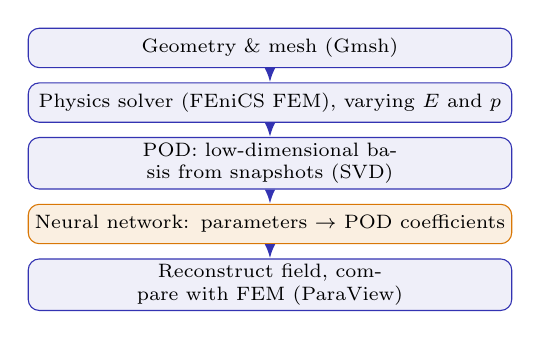
\begin{tikzpicture}[node distance=1.8mm,
  box/.style={draw=qblue,fill=qblue!8,rounded corners,text width=60mm,minimum height=5mm,inner sep=2pt,align=center,font=\scriptsize},
  arr/.style={-{Latex[length=1.8mm]},thick,qblue}]
\node[box] (g) {Geometry \& mesh (Gmsh)};
\node[box,below=of g] (f) {Physics solver (FEniCS FEM), varying $E$ and $p$};
\node[box,below=of f] (p) {POD: low-dimensional basis from snapshots (SVD)};
\node[box,below=of p,draw=qorange,fill=qorange!12] (n) {Neural network: parameters $\to$ POD coefficients};
\node[box,below=of n] (v) {Reconstruct field, compare with FEM (ParaView)};
\draw[arr] (g)--(f); \draw[arr] (f)--(p); \draw[arr] (p)--(n); \draw[arr] (n)--(v);
\end{tikzpicture}
\end{columns}
\takeaway{Same recipe as for crystal growth: simulate a few cases, compress, learn the parameter-to-field map, check against the solver.}
\end{frame}
\optionalfigframe{Cryogenic H$_2$/N$_2$ systems}{cryo_1.jpg}

%============================================================
\section{Dyad Agent (JuliaHub)}
%============================================================
\begin{frame}{Dyad agent: an LLM agent for physical system models}
\begin{columns}[T,onlytextwidth]
\column{0.47\textwidth}
\begin{block}{What Dyad is}
\begin{itemize}\footnotesize
  \item A declarative modelling language from JuliaHub, built on Julia / ModelingToolkit.
  \item Combines physics-based modelling, scientific ML and agentic workflows.
  \item Acausal components with typed connectors (thermal, hydraulic, \dots) enforce conservation at every connection.
\end{itemize}
\end{block}
\begin{exampleblock}{Fit with this work}
\footnotesize Candidate tool for system-level (0D/1D) cryogenic loops (tanks, lines, valves, heat leak), complementing field-level CFD.
\end{exampleblock}
\column{0.50\textwidth}
\centering
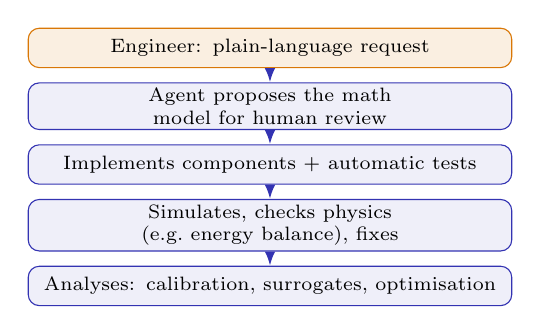
\begin{tikzpicture}[node distance=1.8mm,
  box/.style={draw=qblue,fill=qblue!8,rounded corners,text width=60mm,minimum height=5mm,inner sep=2pt,align=center,font=\scriptsize},
  arr/.style={-{Latex[length=1.8mm]},thick,qblue}]
\node[box,draw=qorange,fill=qorange!12] (a) {Engineer: plain-language request};
\node[box,below=of a] (b) {Agent proposes the math model for human review};
\node[box,below=of b] (c) {Implements components + automatic tests};
\node[box,below=of c] (d) {Simulates, checks physics (e.g.\ energy balance), fixes};
\node[box,below=of d] (e) {Analyses: calibration, surrogates, optimisation};
\draw[arr] (a)--(b); \draw[arr] (b)--(c); \draw[arr] (c)--(d); \draw[arr] (d)--(e);
\end{tikzpicture}
\end{columns}
\takeaway{LLM agents are most trustworthy inside a constrained, checkable language, the same principle as in AutoFOAM.}
\end{frame}
\optionalfigframe{Dyad agent (JuliaHub)}{Dyad.png}

%============================================================
\section{Agentic CFD with AutoFOAM}
%============================================================
\begin{frame}{AutoFOAM: from one sentence to a running OpenFOAM case}
\small An OpenFOAM case is a dozen or more interlinked dictionaries; generic LLMs invent keywords and write inconsistent boundary conditions.
AutoFOAM (fine-tuned 14B model, OpenFOAM v2412) splits the work:
\vspace{2mm}

\centering
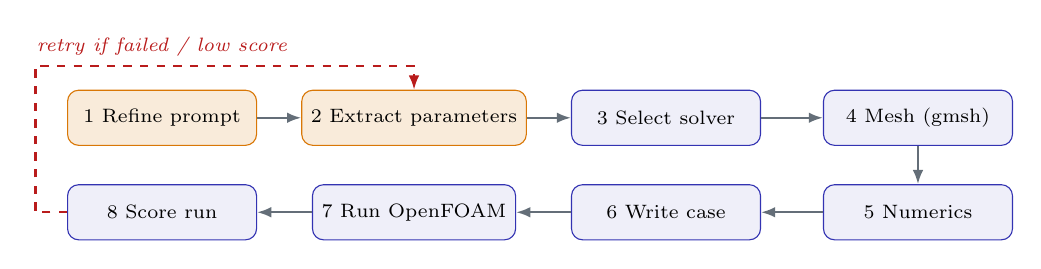
\begin{tikzpicture}[font=\scriptsize,
  llm/.style={draw=qorange,fill=qorange!15,rounded corners,minimum width=24mm,minimum height=7mm,align=center},
  det/.style={draw=qblue,fill=qblue!8,rounded corners,minimum width=24mm,minimum height=7mm,align=center},
  arr/.style={-{Latex[length=1.8mm]},thick,qgray}]
\node[llm] (n1) at (0,0)      {1 Refine prompt};
\node[llm] (n2) at (3.2,0)    {2 Extract parameters};
\node[det] (n3) at (6.4,0)    {3 Select solver};
\node[det] (n4) at (9.6,0)    {4 Mesh (gmsh)};
\node[det] (n5) at (9.6,-1.2) {5 Numerics};
\node[det] (n6) at (6.4,-1.2) {6 Write case};
\node[det] (n7) at (3.2,-1.2) {7 Run OpenFOAM};
\node[det] (n8) at (0,-1.2)   {8 Score run};
\draw[arr] (n1)--(n2); \draw[arr] (n2)--(n3); \draw[arr] (n3)--(n4); \draw[arr] (n4)--(n5);
\draw[arr] (n5)--(n6); \draw[arr] (n6)--(n7); \draw[arr] (n7)--(n8);
\draw[arr,dashed,qred] (n8.west) -- ++(-0.4,0) |- ([yshift=3mm]n2.north) -- (n2.north);
\node[anchor=south,text=qred,font=\scriptsize\itshape] at ([yshift=3mm]n1.north) {retry if failed / low score};
\end{tikzpicture}
\vspace{1mm}

\raggedright
\begin{columns}[T,onlytextwidth]
\column{0.32\textwidth}
\begin{block}{LLM: language}
\footnotesize Understands intent; schema-constrained JSON, so the output always parses.
\end{block}
\column{0.32\textwidth}
\begin{block}{Code: physics decisions}
\footnotesize Rule-based routing to 7 approved solvers; 13 parameterised gmsh geometries.
\end{block}
\column{0.32\textwidth}
\begin{block}{Feedback: self-improving}
\footnotesize Runs are scored; failures are fixed and retried; good runs feed fine-tuning (SFT + DPO).
\end{block}
\end{columns}
\end{frame}

\begin{frame}{AutoFOAM results on 110 unseen prompts}
\begin{columns}[T,onlytextwidth]
\column{0.44\textwidth}
\small
\begin{tabular}{@{}lr@{}}
\toprule
Metric (out-of-distribution) & Value\\
\midrule
Runs without \texttt{FOAM FATAL} error & \textbf{110/110}\\
Execution success & \textbf{100\%}\\
Solver routing accuracy & \textbf{96.4\%}\\
Geometry templates / solver families & 13/13, 7/7\\
Mean run score (0--1) & 0.64\\
\bottomrule
\end{tabular}
\vspace{2mm}
\begin{alertblock}{Caveat}
\small The score rewards convergence: a converged case can still be physically wrong, so a physics validator is the next step.
\end{alertblock}
\column{0.53\textwidth}
\centering
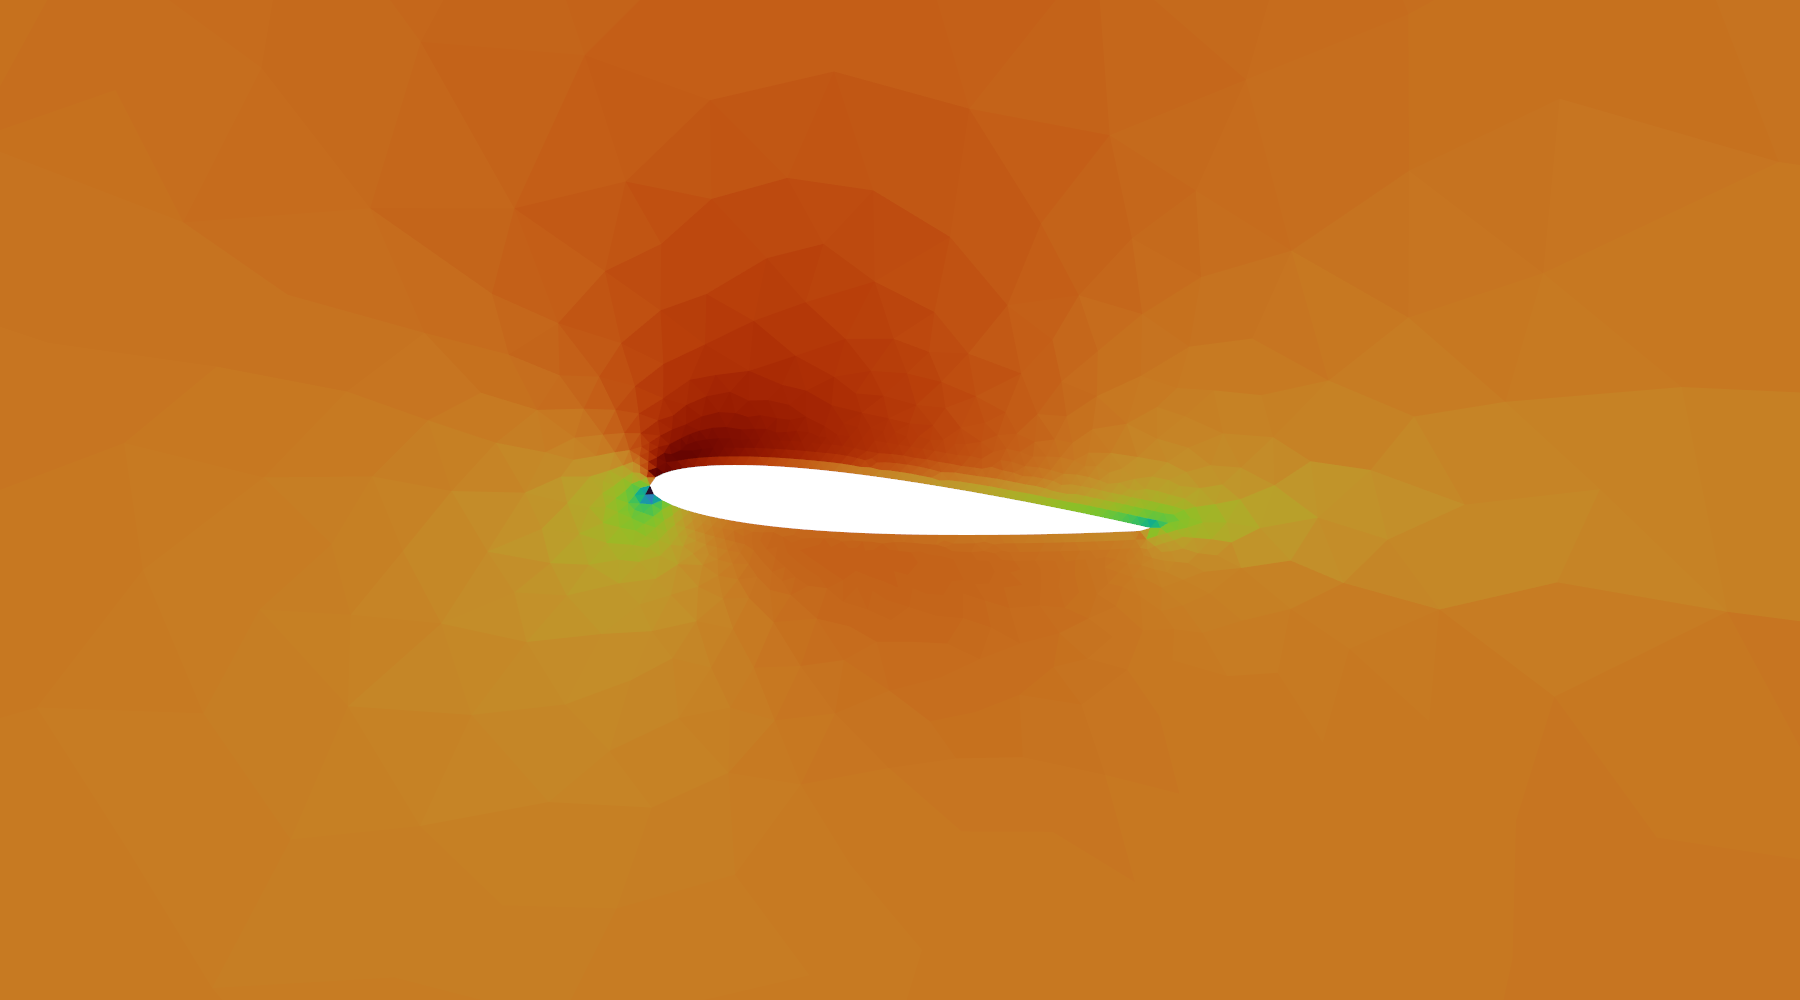
\includegraphics[width=0.49\linewidth,height=1.9cm,keepaspectratio]{airfoil_zoom_mid.png}\hfill
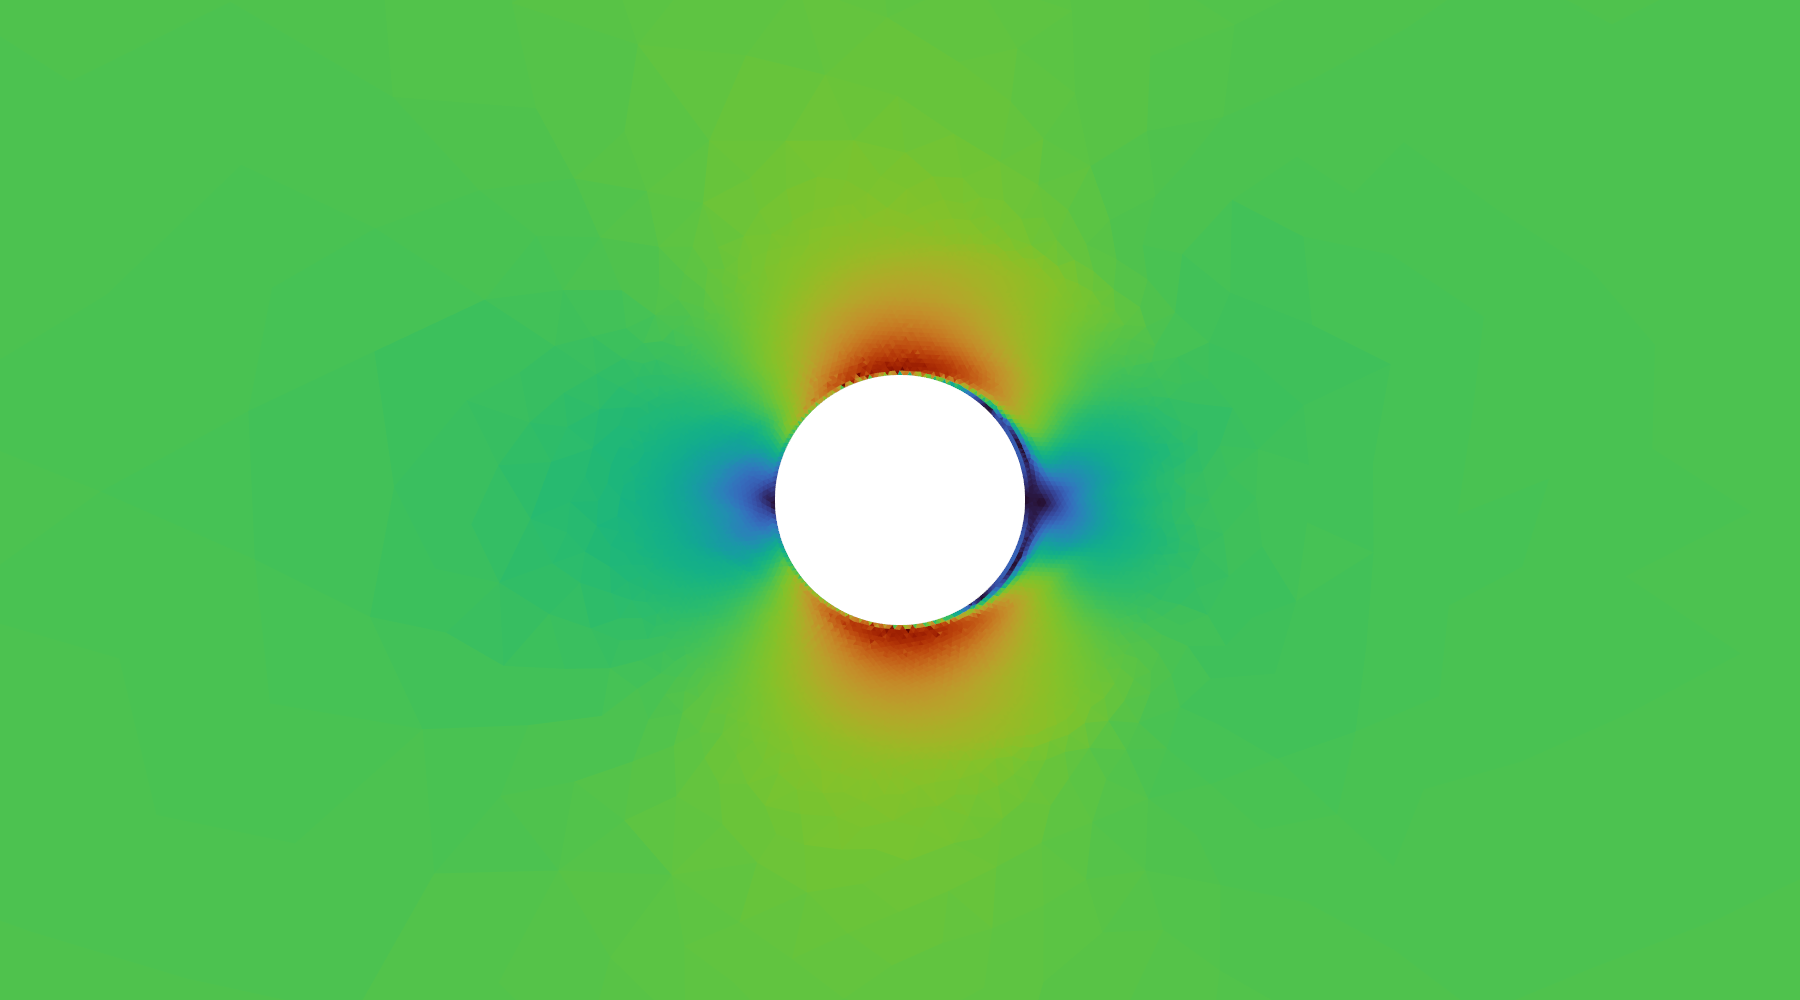
\includegraphics[width=0.49\linewidth,height=1.9cm,keepaspectratio]{cylinder_zoom_mid.png}\\[1mm]
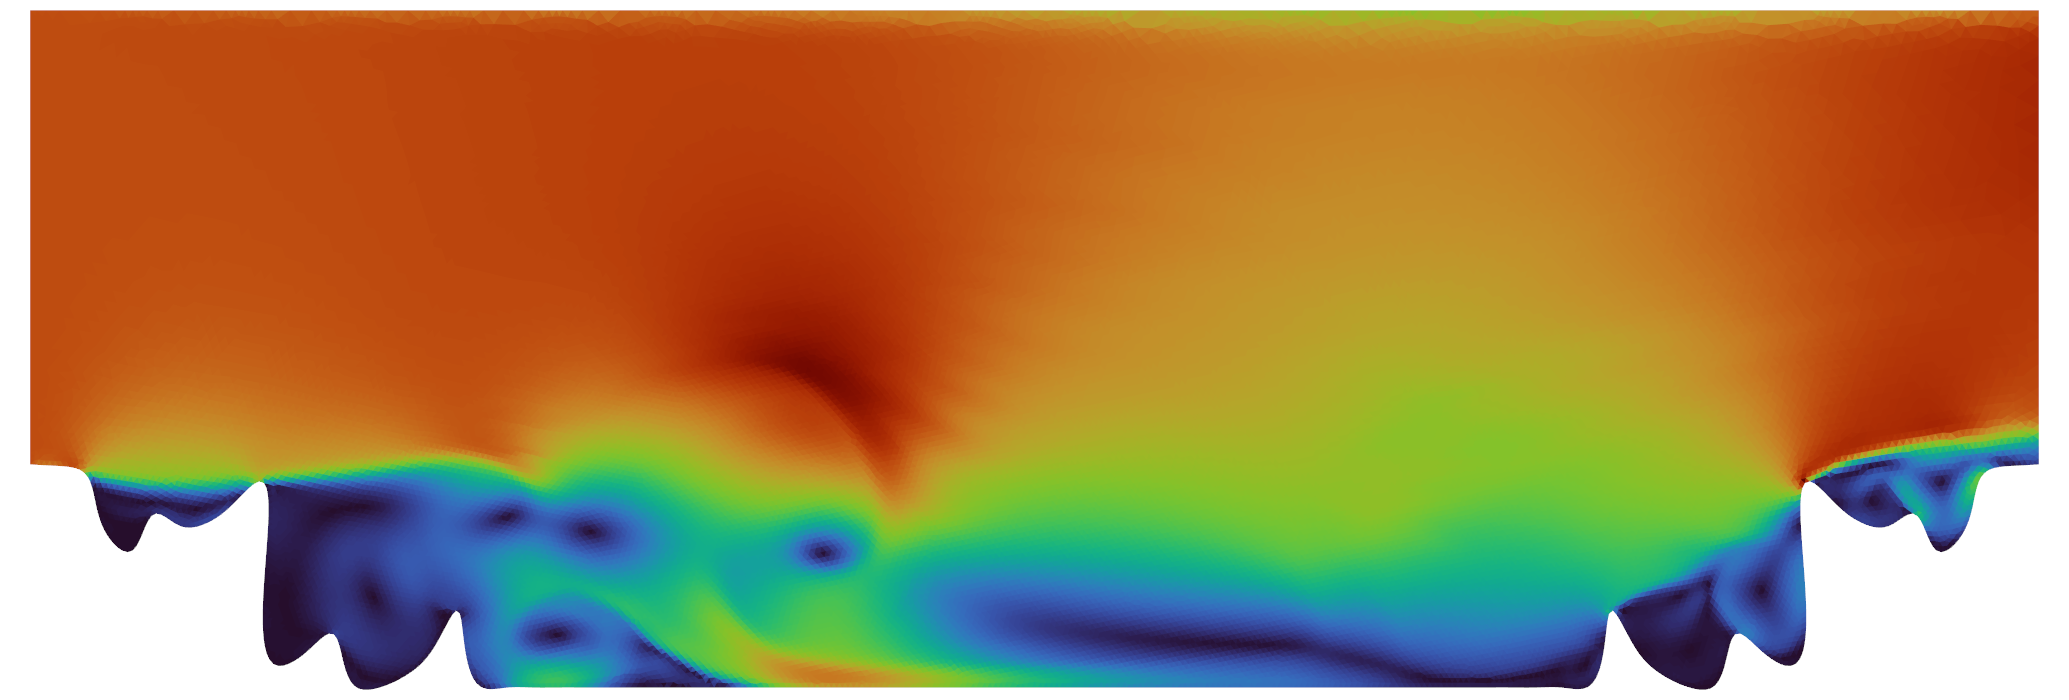
\includegraphics[width=0.62\linewidth,height=1.9cm,keepaspectratio]{clean_periodic_hill_velocity.png}\hfill
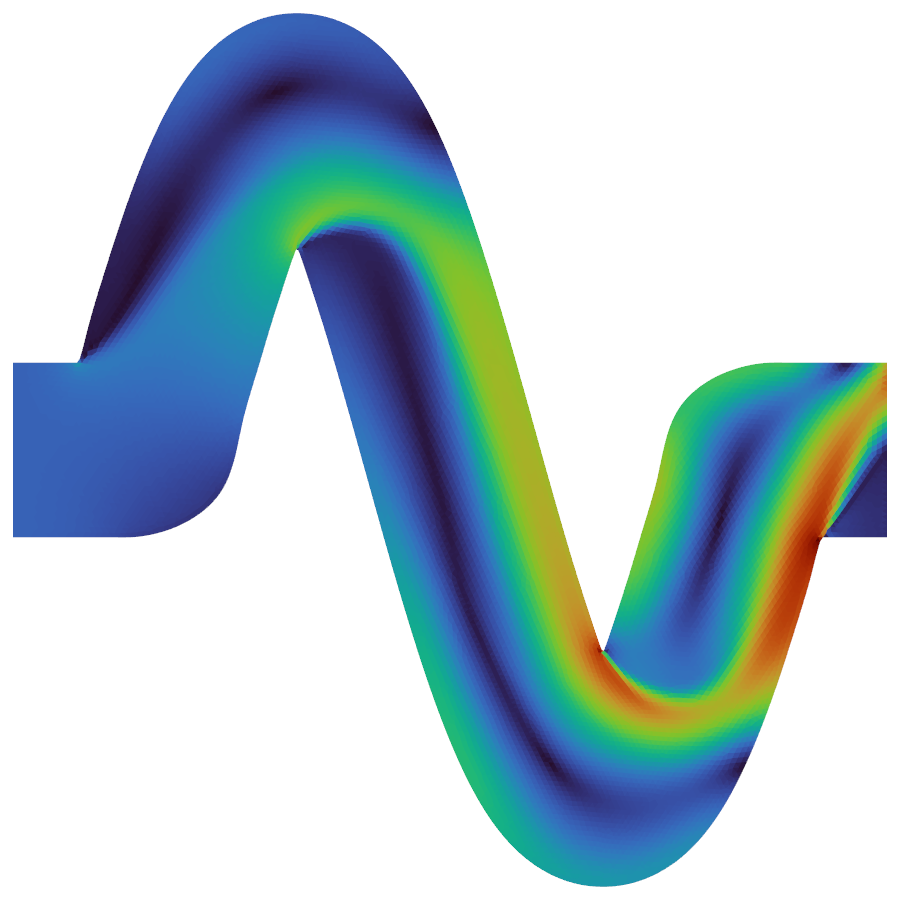
\includegraphics[width=0.33\linewidth,height=1.9cm,keepaspectratio]{clean_sbend_velocity.png}\\[0.5mm]
\figsrc{Velocity fields, each generated from a single prompt: airfoil, cylinder, periodic hill, S-bend}\\[0.5mm]
\scriptsize Demo: \weblink{https://www.youtube.com/watch?v=Kx17bfFlMSc}{youtu.be/Kx17bfFlMSc}\\
Code: \weblink{https://github.com/AGN000/AutoFOAM}{github.com/AGN000/AutoFOAM}
\end{columns}
\end{frame}

%============================================================
\section{Summary and Outlook}
%============================================================
\begin{frame}{Key takeaways and next steps}
\begin{columns}[T,onlytextwidth]
\column{0.58\textwidth}
\begin{enumerate}\small\setlength{\itemsep}{3pt}
  \item \key{Objective $\neq$ accuracy:} a PINN can cut its PDE residual 4800$\times$ and still give the wrong field. Report PDE, BC and IC terms separately.
  \item \key{Error is field-specific:} the CZ surrogate predicts temperature within 10\% but axial velocity only within 41\%.
  \item \key{Agents remove set-up friction:} AutoFOAM runs 110/110 unseen prompts; Dyad builds checked system models.
  \item \key{Validation is the common layer:} neither a low loss nor a converged run is proof on its own.
\end{enumerate}
\column{0.38\textwidth}
\begin{block}{Next steps}
\begin{itemize}\small
  \item More PDEs and random seeds; higher-fidelity CZ models.
  \item Thermal (heat-leak) surrogates for cryogenic vessels.
  \item A physics validator inside the agent loop.
\end{itemize}
\end{block}
\end{columns}
\takeaway{Physics-informed surrogates + agentic automation + explicit validation $\Rightarrow$ fast, accessible and trustworthy CFD.}
\end{frame}

%============================================================
\section{Acknowledgments}
%============================================================
\begin{frame}{Acknowledgments}
\small This talk presents the joint work of:\\[2mm]
\renewcommand{\arraystretch}{1.3}
\begin{tabularx}{\textwidth}{@{}>{\bfseries}l L@{}}
\toprule
Niruta Chapagain, Rohit Raj & Adaptive PINN study for crystal growth (NeurIPS 2026 Sim2Science workshop paper) \\
Bertwin Kurisinkal Shine (TU Chemnitz) & CZ reference CFD: ANSYS Fluent set-up, parameter sweeps, mesh-independence study and certification \\
Arun Govind Neelan & AutoFOAM: agent design, fine-tuned model, training data and evaluation \\
A Seshaditya (QuaSi, Berlin) & Physics-informed ML project; AutoFOAM co-author \\
\bottomrule
\end{tabularx}
\vspace{2mm}

\footnotesize We also thank JuliaHub (Dyad) and the OpenFOAM, Gmsh and FEniCS communities. The CZ geometry and boundary conditions follow Huang et al.\ (2025).
\vfill
\centering
{\Large\textcolor{qblue}{\textbf{Thank you! Questions?}}}\\[1mm]
\footnotesize\weblink{https://quasi.digital}{quasi.digital}\quad
\weblink{https://github.com/adytiaa/quasi.ai}{github.com/adytiaa/quasi.ai}
\vspace{2mm}
\end{frame}

\section*{References}
\begin{frame}{Selected references}
\scriptsize
\begin{itemize}\setlength{\itemsep}{2pt}
  \item M.~Raissi, P.~Perdikaris, G.~E.~Karniadakis (2019). Physics-informed neural networks. \emph{J.\ Comput.\ Phys.} 378, 686--707.
  \item S.~Wang, Y.~Teng, P.~Perdikaris (2021). Understanding and mitigating gradient flow pathologies in PINNs. \emph{SIAM J.\ Sci.\ Comput.} 43, A3055--A3081.
  \item W.~Huang, S.~Cao, R.~Liu, D.~Liu (2025). Thermal-fluid coupling in Czochralski silicon growth based on an improved PINN. \emph{AIP Advances} 15, 105202. doi:10.1063/5.0271778.
  \item N.~Chapagain et al.\ (2026). Component-level evaluation of adaptive PINN training for CFD-oriented crystal growth simulation. NeurIPS 2026 Sim2Science workshop.
  \item A.~G.~Neelan, A.~Seshaditya. AutoFOAM: the self-refining autonomous OpenFOAM agent. \weblink{https://github.com/AGN000/AutoFOAM}{github.com/AGN000/AutoFOAM}.
  \item JuliaHub. Dyad documentation and AI agent. \weblink{https://help.juliahub.com/dyad/stable/}{help.juliahub.com/dyad}.
\end{itemize}
\end{frame}

\end{document}
